\documentclass[1p]{elsarticle_modified}
%\bibliographystyle{elsarticle-num}

%\usepackage[colorlinks]{hyperref}
%\usepackage{abbrmath_seonhwa} %\Abb, \Ascr, \Acal ,\Abf, \Afrak
\usepackage{amsfonts}
\usepackage{amssymb}
\usepackage{amsmath}
\usepackage{amsthm}
\usepackage{scalefnt}
\usepackage{amsbsy}
\usepackage{kotex}
\usepackage{caption}
\usepackage{subfig}
\usepackage{color}
\usepackage{graphicx}
\usepackage{xcolor} %% white, black, red, green, blue, cyan, magenta, yellow
\usepackage{float}
\usepackage{setspace}
\usepackage{hyperref}

\usepackage{tikz}
\usetikzlibrary{arrows}

\usepackage{multirow}
\usepackage{array} % fixed length table
\usepackage{hhline}

%%%%%%%%%%%%%%%%%%%%%
\makeatletter
\renewcommand*\env@matrix[1][\arraystretch]{%
	\edef\arraystretch{#1}%
	\hskip -\arraycolsep
	\let\@ifnextchar\new@ifnextchar
	\array{*\c@MaxMatrixCols c}}
\makeatother %https://tex.stackexchange.com/questions/14071/how-can-i-increase-the-line-spacing-in-a-matrix
%%%%%%%%%%%%%%%

\usepackage[normalem]{ulem}

\newcommand{\msout}[1]{\ifmmode\text{\sout{\ensuremath{#1}}}\else\sout{#1}\fi}
%SOURCE: \msout is \stkout macro in https://tex.stackexchange.com/questions/20609/strikeout-in-math-mode

\newcommand{\cancel}[1]{
	\ifmmode
	{\color{red}\msout{#1}}
	\else
	{\color{red}\sout{#1}}
	\fi
}

\newcommand{\add}[1]{
	{\color{blue}\uwave{#1}}
}

\newcommand{\replace}[2]{
	\ifmmode
	{\color{red}\msout{#1}}{\color{blue}\uwave{#2}}
	\else
	{\color{red}\sout{#1}}{\color{blue}\uwave{#2}}
	\fi
}

\newcommand{\Sol}{\mathcal{S}} %segment
\newcommand{\D}{D} %diagram
\newcommand{\A}{\mathcal{A}} %arc


%%%%%%%%%%%%%%%%%%%%%%%%%%%%%5 test

\def\sl{\operatorname{\textup{SL}}(2,\Cbb)}
\def\psl{\operatorname{\textup{PSL}}(2,\Cbb)}
\def\quan{\mkern 1mu \triangleright \mkern 1mu}

\theoremstyle{definition}
\newtheorem{thm}{Theorem}[section]
\newtheorem{prop}[thm]{Proposition}
\newtheorem{lem}[thm]{Lemma}
\newtheorem{ques}[thm]{Question}
\newtheorem{cor}[thm]{Corollary}
\newtheorem{defn}[thm]{Definition}
\newtheorem{exam}[thm]{Example}
\newtheorem{rmk}[thm]{Remark}
\newtheorem{alg}[thm]{Algorithm}

\newcommand{\I}{\sqrt{-1}}
\begin{document}

%\begin{frontmatter}
%
%\title{Boundary parabolic representations of knots up to 8 crossings}
%
%%% Group authors per affiliation:
%\author{Yunhi Cho} 
%\address{Department of Mathematics, University of Seoul, Seoul, Korea}
%\ead{yhcho@uos.ac.kr}
%
%
%\author{Seonhwa Kim} %\fnref{s_kim}}
%\address{Center for Geometry and Physics, Institute for Basic Science, Pohang, 37673, Korea}
%\ead{ryeona17@ibs.re.kr}
%
%\author{Hyuk Kim}
%\address{Department of Mathematical Sciences, Seoul National University, Seoul 08826, Korea}
%\ead{hyukkim@snu.ac.kr}
%
%\author{Seokbeom Yoon}
%\address{Department of Mathematical Sciences, Seoul National University, Seoul, 08826,  Korea}
%\ead{sbyoon15@snu.ac.kr}
%
%\begin{abstract}
%We find all boundary parabolic representation of knots up to 8 crossings.
%
%\end{abstract}
%\begin{keyword}
%    \MSC[2010] 57M25 
%\end{keyword}
%
%\end{frontmatter}

%\linenumbers
%\tableofcontents
%
\newcommand\colored[1]{\textcolor{white}{\rule[-0.35ex]{0.8em}{1.4ex}}\kern-0.8em\color{red} #1}%
%\newcommand\colored[1]{\textcolor{white}{ #1}\kern-2.17ex	\textcolor{white}{ #1}\kern-1.81ex	\textcolor{white}{ #1}\kern-2.15ex\color{red}#1	}

{\Large $\underline{12n_{0014}~(K12n_{0014})}$}

\setlength{\tabcolsep}{10pt}
\renewcommand{\arraystretch}{1.6}
\vspace{1cm}\begin{tabular}{m{100pt}>{\centering\arraybackslash}m{274pt}}
\multirow{5}{120pt}{
	\centering
	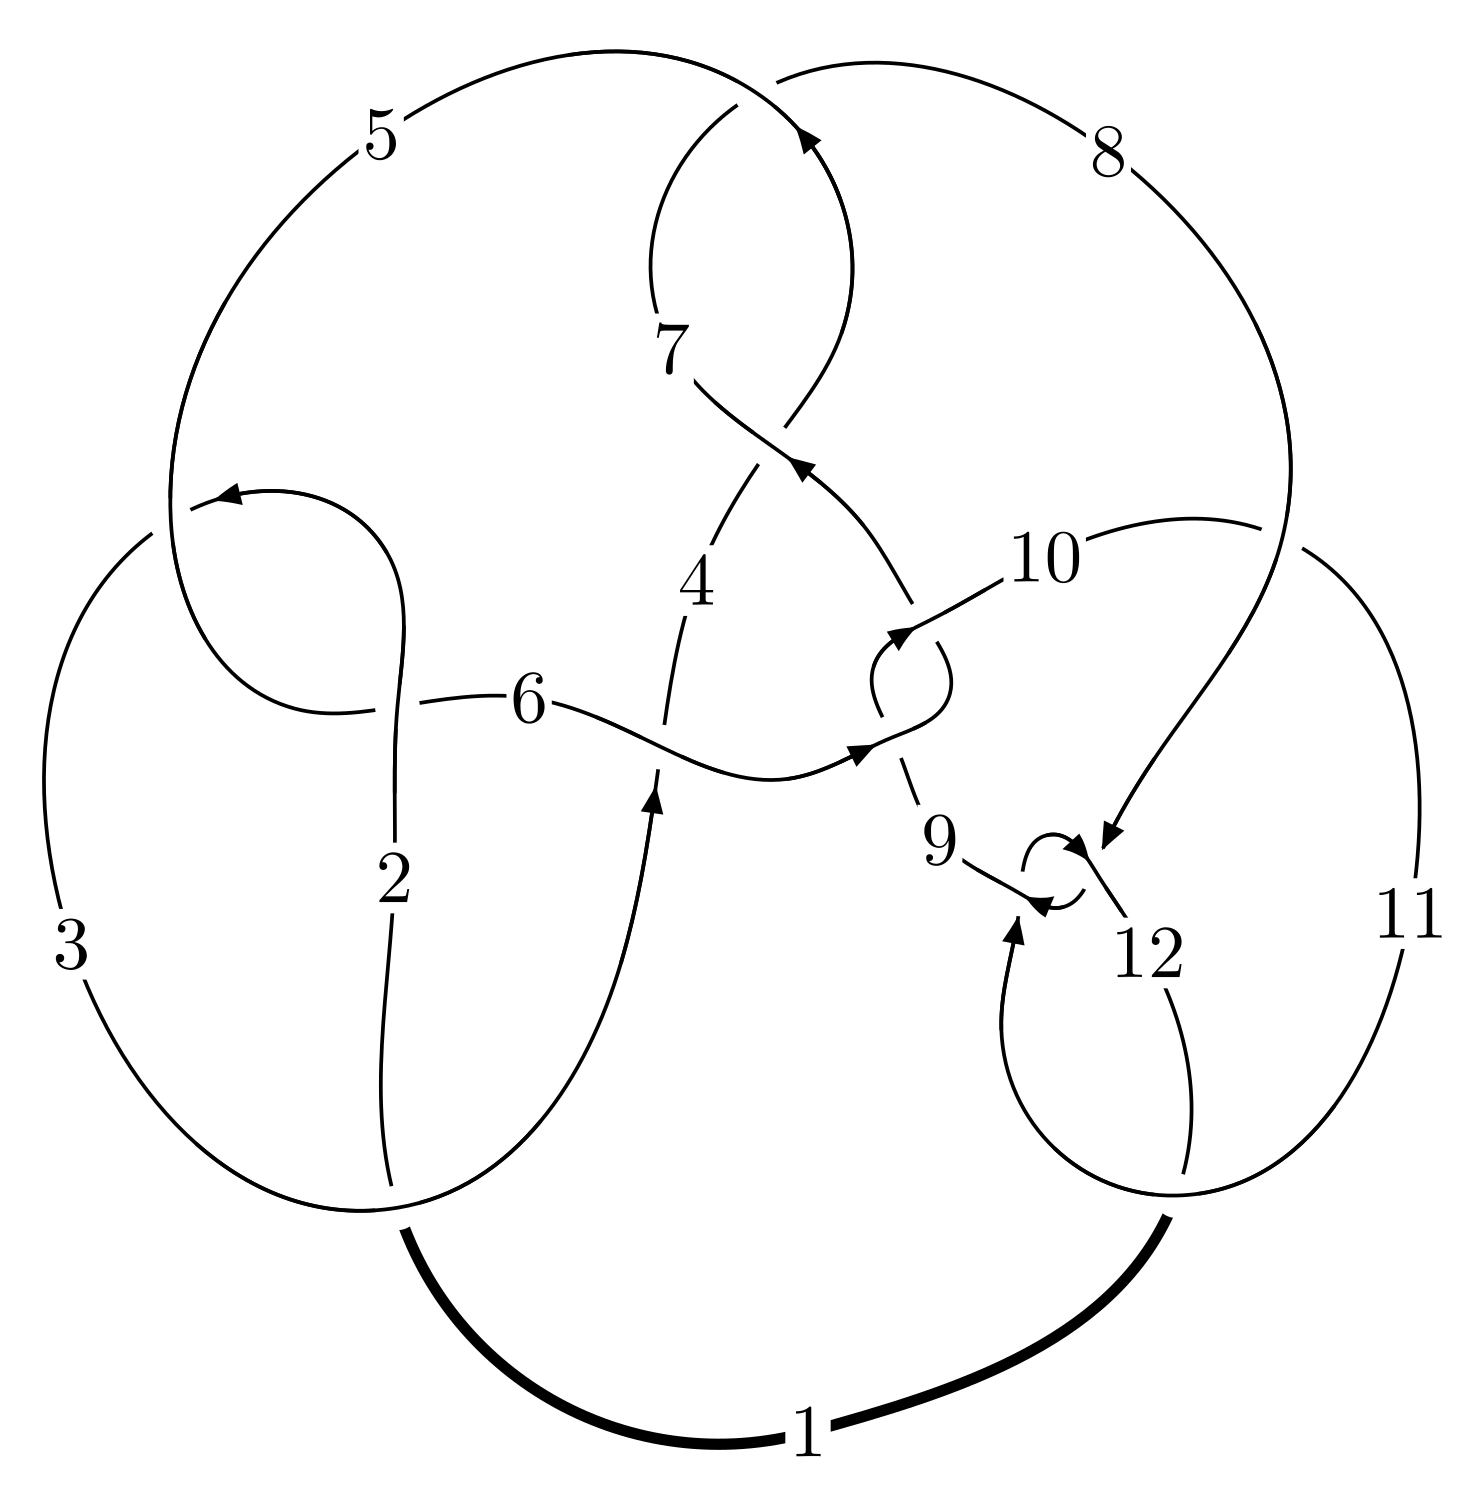
\includegraphics[width=112pt]{../../../GIT/diagram.site/Diagrams/png/2103_12n_0014.png}\\
\ \ \ A knot diagram\footnotemark}&
\allowdisplaybreaks
\textbf{Linearized knot diagam} \\
\cline{2-2}
 &
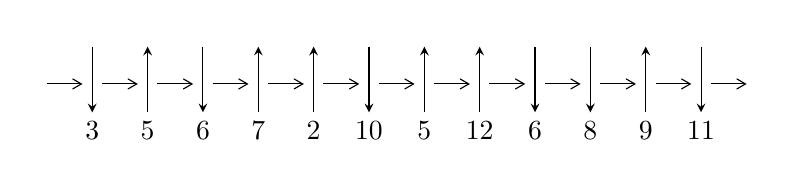
\begin{tikzpicture}[x=20pt, y=17pt]
	% nodes
	\node (C0) at (0, 0) {};
	\node (C1) at (1, 0) {};
	\node (C1U) at (1, +1) {};
	\node (C1D) at (1, -1) {3};

	\node (C2) at (2, 0) {};
	\node (C2U) at (2, +1) {};
	\node (C2D) at (2, -1) {5};

	\node (C3) at (3, 0) {};
	\node (C3U) at (3, +1) {};
	\node (C3D) at (3, -1) {6};

	\node (C4) at (4, 0) {};
	\node (C4U) at (4, +1) {};
	\node (C4D) at (4, -1) {7};

	\node (C5) at (5, 0) {};
	\node (C5U) at (5, +1) {};
	\node (C5D) at (5, -1) {2};

	\node (C6) at (6, 0) {};
	\node (C6U) at (6, +1) {};
	\node (C6D) at (6, -1) {10};

	\node (C7) at (7, 0) {};
	\node (C7U) at (7, +1) {};
	\node (C7D) at (7, -1) {5};

	\node (C8) at (8, 0) {};
	\node (C8U) at (8, +1) {};
	\node (C8D) at (8, -1) {12};

	\node (C9) at (9, 0) {};
	\node (C9U) at (9, +1) {};
	\node (C9D) at (9, -1) {6};

	\node (C10) at (10, 0) {};
	\node (C10U) at (10, +1) {};
	\node (C10D) at (10, -1) {8};

	\node (C11) at (11, 0) {};
	\node (C11U) at (11, +1) {};
	\node (C11D) at (11, -1) {9};

	\node (C12) at (12, 0) {};
	\node (C12U) at (12, +1) {};
	\node (C12D) at (12, -1) {11};
	\node (C13) at (13, 0) {};

	% arrows
	\draw[->,>={angle 60}]
	(C0) edge (C1) (C1) edge (C2) (C2) edge (C3) (C3) edge (C4) (C4) edge (C5) (C5) edge (C6) (C6) edge (C7) (C7) edge (C8) (C8) edge (C9) (C9) edge (C10) (C10) edge (C11) (C11) edge (C12) (C12) edge (C13) ;	\draw[->,>=stealth]
	(C1U) edge (C1D) (C2D) edge (C2U) (C3U) edge (C3D) (C4D) edge (C4U) (C5D) edge (C5U) (C6U) edge (C6D) (C7D) edge (C7U) (C8D) edge (C8U) (C9U) edge (C9D) (C10U) edge (C10D) (C11D) edge (C11U) (C12U) edge (C12D) ;
	\end{tikzpicture} \\
\hhline{~~} \\& 
\textbf{Solving Sequence} \\ \cline{2-2} 
 &
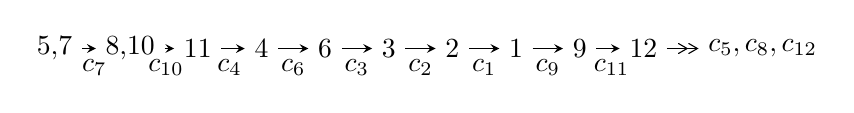
\begin{tikzpicture}[x=23pt, y=7pt]
	% node
	\node (A0) at (-1/8, 0) {5,7};
	\node (A1) at (17/16, 0) {8,10};
	\node (A2) at (17/8, 0) {11};
	\node (A3) at (25/8, 0) {4};
	\node (A4) at (33/8, 0) {6};
	\node (A5) at (41/8, 0) {3};
	\node (A6) at (49/8, 0) {2};
	\node (A7) at (57/8, 0) {1};
	\node (A8) at (65/8, 0) {9};
	\node (A9) at (73/8, 0) {12};
	\node (C1) at (1/2, -1) {$c_{7}$};
	\node (C2) at (13/8, -1) {$c_{10}$};
	\node (C3) at (21/8, -1) {$c_{4}$};
	\node (C4) at (29/8, -1) {$c_{6}$};
	\node (C5) at (37/8, -1) {$c_{3}$};
	\node (C6) at (45/8, -1) {$c_{2}$};
	\node (C7) at (53/8, -1) {$c_{1}$};
	\node (C8) at (61/8, -1) {$c_{9}$};
	\node (C9) at (69/8, -1) {$c_{11}$};
	\node (A10) at (11, 0) {$c_{5},c_{8},c_{12}$};

	% edge
	\draw[->,>=stealth]	
	(A0) edge (A1) (A1) edge (A2) (A2) edge (A3) (A3) edge (A4) (A4) edge (A5) (A5) edge (A6) (A6) edge (A7) (A7) edge (A8) (A8) edge (A9) ;
	\draw[->>,>={angle 60}]	
	(A9) edge (A10);
\end{tikzpicture} \\ 

\end{tabular} \\

\footnotetext{
The image of knot diagram is generated by the software ``\textbf{Draw programme}" developed by Andrew Bartholomew(\url{http://www.layer8.co.uk/maths/draw/index.htm\#Running-draw}), where we modified some parts for our purpose(\url{https://github.com/CATsTAILs/LinksPainter}).
}\phantom \\ \newline 
\centering \textbf{Ideals for irreducible components\footnotemark of $X_{\text{par}}$} 
 
\begin{align*}
I^u_{1}&=\langle 
-3.93906\times10^{169} u^{53}+8.11692\times10^{169} u^{52}+\cdots+2.56580\times10^{172} b+5.59119\times10^{173},\\
\phantom{I^u_{1}}&\phantom{= \langle  }2.70535\times10^{172} u^{53}+1.41390\times10^{173} u^{52}+\cdots+1.43685\times10^{174} a+5.91275\times10^{175},\\
\phantom{I^u_{1}}&\phantom{= \langle  }u^{54}+5 u^{53}+\cdots+2048 u+1024\rangle \\
\\
I^v_{1}&=\langle 
a,\;8286 v^9-14092 v^8+\cdots+8095 b+12581,\\
\phantom{I^v_{1}}&\phantom{= \langle  }v^{10}- v^9-2 v^8-19 v^7+12 v^6+35 v^5+50 v^4+34 v^3+17 v^2+5 v+1\rangle \\
\end{align*}
\raggedright * 2 irreducible components of $\dim_{\mathbb{C}}=0$, with total 64 representations.\\
\footnotetext{All coefficients of polynomials are rational numbers. But the coefficients are sometimes approximated in decimal forms when there is not enough margin.}
\newpage
\renewcommand{\arraystretch}{1}
\centering \section*{I. $I^u_{1}= \langle -3.94\times10^{169} u^{53}+8.12\times10^{169} u^{52}+\cdots+2.57\times10^{172} b+5.59\times10^{173},\;2.71\times10^{172} u^{53}+1.41\times10^{173} u^{52}+\cdots+1.44\times10^{174} a+5.91\times10^{175},\;u^{54}+5 u^{53}+\cdots+2048 u+1024 \rangle$}
\flushleft \textbf{(i) Arc colorings}\\
\begin{tabular}{m{7pt} m{180pt} m{7pt} m{180pt} }
\flushright $a_{5}=$&$\begin{pmatrix}0\\u\end{pmatrix}$ \\
\flushright $a_{7}=$&$\begin{pmatrix}1\\0\end{pmatrix}$ \\
\flushright $a_{8}=$&$\begin{pmatrix}1\\- u^2\end{pmatrix}$ \\
\flushright $a_{10}=$&$\begin{pmatrix}-0.0188284 u^{53}-0.0984027 u^{52}+\cdots-57.6613 u-41.1508\\0.00153522 u^{53}-0.00316351 u^{52}+\cdots+2.45774 u-21.7912\end{pmatrix}$ \\
\flushright $a_{11}=$&$\begin{pmatrix}-0.0323517 u^{53}-0.147501 u^{52}+\cdots-88.1255 u-23.7227\\0.0109343 u^{53}+0.0438860 u^{52}+\cdots+26.5354 u-2.82844\end{pmatrix}$ \\
\flushright $a_{4}=$&$\begin{pmatrix}- u\\u\end{pmatrix}$ \\
\flushright $a_{6}=$&$\begin{pmatrix}-0.0118561 u^{53}-0.0590764 u^{52}+\cdots-36.2368 u-21.2553\\0.0134039 u^{53}+0.0620483 u^{52}+\cdots+36.4660 u+13.4608\end{pmatrix}$ \\
\flushright $a_{3}=$&$\begin{pmatrix}0.00441031 u^{53}+0.0172727 u^{52}+\cdots+10.8004 u-5.96037\\0.00533450 u^{53}+0.0282151 u^{52}+\cdots+13.6825 u+15.5729\end{pmatrix}$ \\
\flushright $a_{2}=$&$\begin{pmatrix}0.00441031 u^{53}+0.0172727 u^{52}+\cdots+10.8004 u-5.96037\\0.00669340 u^{53}+0.0361984 u^{52}+\cdots+18.9533 u+20.4664\end{pmatrix}$ \\
\flushright $a_{1}=$&$\begin{pmatrix}-0.00154779 u^{53}-0.00297199 u^{52}+\cdots-0.229176 u+7.79450\\0.0169009 u^{53}+0.0786020 u^{52}+\cdots+44.6438 u+18.3421\end{pmatrix}$ \\
\flushright $a_{9}=$&$\begin{pmatrix}-0.00933751 u^{53}-0.0594844 u^{52}+\cdots-30.9568 u-43.0824\\-0.0225428 u^{53}-0.0990264 u^{52}+\cdots-54.4975 u-12.8121\end{pmatrix}$ \\
\flushright $a_{12}=$&$\begin{pmatrix}-0.0399571 u^{53}-0.175227 u^{52}+\cdots-100.366 u-19.0531\\0.00625323 u^{53}+0.0325196 u^{52}+\cdots+12.5340 u+17.1289\end{pmatrix}$\\&\end{tabular}
\flushleft \textbf{(ii) Obstruction class $= -1$}\\~\\
\flushleft \textbf{(iii) Cusp Shapes $= -0.00845297 u^{53}-0.0644904 u^{52}+\cdots-23.1790 u-60.4595$}\\~\\
\newpage\renewcommand{\arraystretch}{1}
\flushleft \textbf{(iv) u-Polynomials at the component}\newline \\
\begin{tabular}{m{50pt}|m{274pt}}
Crossings & \hspace{64pt}u-Polynomials at each crossing \\
\hline $$\begin{aligned}c_{1}\end{aligned}$$&$\begin{aligned}
&u^{54}+14 u^{53}+\cdots-53 u+1
\end{aligned}$\\
\hline $$\begin{aligned}c_{2},c_{5}\end{aligned}$$&$\begin{aligned}
&u^{54}+6 u^{53}+\cdots+15 u+1
\end{aligned}$\\
\hline $$\begin{aligned}c_{3}\end{aligned}$$&$\begin{aligned}
&u^{54}-6 u^{53}+\cdots+11895099 u+596177
\end{aligned}$\\
\hline $$\begin{aligned}c_{4},c_{7}\end{aligned}$$&$\begin{aligned}
&u^{54}+5 u^{53}+\cdots+2048 u+1024
\end{aligned}$\\
\hline $$\begin{aligned}c_{6},c_{9}\end{aligned}$$&$\begin{aligned}
&u^{54}+3 u^{53}+\cdots+4 u^2+1
\end{aligned}$\\
\hline $$\begin{aligned}c_{8},c_{11}\end{aligned}$$&$\begin{aligned}
&u^{54}+3 u^{53}+\cdots-2 u+1
\end{aligned}$\\
\hline $$\begin{aligned}c_{10}\end{aligned}$$&$\begin{aligned}
&u^{54}-3 u^{53}+\cdots-8544 u+1217
\end{aligned}$\\
\hline $$\begin{aligned}c_{12}\end{aligned}$$&$\begin{aligned}
&u^{54}+23 u^{53}+\cdots+8 u+1
\end{aligned}$\\
\hline
\end{tabular}\\~\\
\newpage\renewcommand{\arraystretch}{1}
\flushleft \textbf{(v) Riley Polynomials at the component}\newline \\
\begin{tabular}{m{50pt}|m{274pt}}
Crossings & \hspace{64pt}Riley Polynomials at each crossing \\
\hline $$\begin{aligned}c_{1}\end{aligned}$$&$\begin{aligned}
&y^{54}+58 y^{53}+\cdots+2411 y+1
\end{aligned}$\\
\hline $$\begin{aligned}c_{2},c_{5}\end{aligned}$$&$\begin{aligned}
&y^{54}+14 y^{53}+\cdots-53 y+1
\end{aligned}$\\
\hline $$\begin{aligned}c_{3}\end{aligned}$$&$\begin{aligned}
&y^{54}+102 y^{53}+\cdots-14429377332621 y+355427015329
\end{aligned}$\\
\hline $$\begin{aligned}c_{4},c_{7}\end{aligned}$$&$\begin{aligned}
&y^{54}-55 y^{53}+\cdots-4194304 y+1048576
\end{aligned}$\\
\hline $$\begin{aligned}c_{6},c_{9}\end{aligned}$$&$\begin{aligned}
&y^{54}-5 y^{53}+\cdots+8 y+1
\end{aligned}$\\
\hline $$\begin{aligned}c_{8},c_{11}\end{aligned}$$&$\begin{aligned}
&y^{54}+23 y^{53}+\cdots+8 y+1
\end{aligned}$\\
\hline $$\begin{aligned}c_{10}\end{aligned}$$&$\begin{aligned}
&y^{54}+15 y^{53}+\cdots+18080344 y+1481089
\end{aligned}$\\
\hline $$\begin{aligned}c_{12}\end{aligned}$$&$\begin{aligned}
&y^{54}+19 y^{53}+\cdots-160 y+1
\end{aligned}$\\
\hline
\end{tabular}\\~\\
\newpage\flushleft \textbf{(vi) Complex Volumes and Cusp Shapes}
$$\begin{array}{c|c|c}  
\text{Solutions to }I^u_{1}& \I (\text{vol} + \sqrt{-1}CS) & \text{Cusp shape}\\
 \hline 
\begin{aligned}
u &= -0.968225 + 0.607102 I \\
a &= -0.164875 - 0.865628 I \\
b &= \phantom{-}0.789588 + 0.453320 I\end{aligned}
 & -3.62207 - 1.88435 I & \phantom{-0.000000 } 0 \\ \hline\begin{aligned}
u &= -0.968225 - 0.607102 I \\
a &= -0.164875 + 0.865628 I \\
b &= \phantom{-}0.789588 - 0.453320 I\end{aligned}
 & -3.62207 + 1.88435 I & \phantom{-0.000000 } 0 \\ \hline\begin{aligned}
u &= \phantom{-}0.556588 + 0.619363 I \\
a &= \phantom{-}0.901194 + 0.566536 I \\
b &= \phantom{-}0.051996 - 0.642624 I\end{aligned}
 & \phantom{-}0.99939 + 1.40813 I & \phantom{-}3.91416 - 3.69919 I \\ \hline\begin{aligned}
u &= \phantom{-}0.556588 - 0.619363 I \\
a &= \phantom{-}0.901194 - 0.566536 I \\
b &= \phantom{-}0.051996 + 0.642624 I\end{aligned}
 & \phantom{-}0.99939 - 1.40813 I & \phantom{-}3.91416 + 3.69919 I \\ \hline\begin{aligned}
u &= -0.661385 + 0.335932 I \\
a &= \phantom{-}1.52538 - 0.28332 I \\
b &= -0.395578 + 0.434236 I\end{aligned}
 & -0.24598 + 2.82121 I & \phantom{-}1.02280 - 2.27971 I \\ \hline\begin{aligned}
u &= -0.661385 - 0.335932 I \\
a &= \phantom{-}1.52538 + 0.28332 I \\
b &= -0.395578 - 0.434236 I\end{aligned}
 & -0.24598 - 2.82121 I & \phantom{-}1.02280 + 2.27971 I \\ \hline\begin{aligned}
u &= -0.569346 + 0.474090 I \\
a &= \phantom{-}1.99530 - 0.80720 I \\
b &= \phantom{-}0.663565 - 0.017228 I\end{aligned}
 & \phantom{-}0.611788 + 1.006080 I & -3.88173 - 0.39430 I \\ \hline\begin{aligned}
u &= -0.569346 - 0.474090 I \\
a &= \phantom{-}1.99530 + 0.80720 I \\
b &= \phantom{-}0.663565 + 0.017228 I\end{aligned}
 & \phantom{-}0.611788 - 1.006080 I & -3.88173 + 0.39430 I \\ \hline\begin{aligned}
u &= \phantom{-}0.511621 + 0.452929 I \\
a &= -0.55984 - 1.59306 I \\
b &= \phantom{-}0.023415 + 0.808214 I\end{aligned}
 & -1.18484 - 1.48546 I & -2.98046 + 1.14168 I \\ \hline\begin{aligned}
u &= \phantom{-}0.511621 - 0.452929 I \\
a &= -0.55984 + 1.59306 I \\
b &= \phantom{-}0.023415 - 0.808214 I\end{aligned}
 & -1.18484 + 1.48546 I & -2.98046 - 1.14168 I\\
 \hline 
 \end{array}$$\newpage$$\begin{array}{c|c|c}  
\text{Solutions to }I^u_{1}& \I (\text{vol} + \sqrt{-1}CS) & \text{Cusp shape}\\
 \hline 
\begin{aligned}
u &= -0.423245 + 0.528845 I \\
a &= \phantom{-}0.207901 + 0.031710 I \\
b &= \phantom{-}1.208630 - 0.192759 I\end{aligned}
 & -2.63355 + 1.15153 I & -2.76262 + 2.47931 I \\ \hline\begin{aligned}
u &= -0.423245 - 0.528845 I \\
a &= \phantom{-}0.207901 - 0.031710 I \\
b &= \phantom{-}1.208630 + 0.192759 I\end{aligned}
 & -2.63355 - 1.15153 I & -2.76262 - 2.47931 I \\ \hline\begin{aligned}
u &= -0.362967 + 0.571541 I \\
a &= \phantom{-}0.026420 + 0.236077 I \\
b &= -1.351430 - 0.085409 I\end{aligned}
 & -6.34508 - 2.87510 I & -9.60101 + 6.45832 I \\ \hline\begin{aligned}
u &= -0.362967 - 0.571541 I \\
a &= \phantom{-}0.026420 - 0.236077 I \\
b &= -1.351430 + 0.085409 I\end{aligned}
 & -6.34508 + 2.87510 I & -9.60101 - 6.45832 I \\ \hline\begin{aligned}
u &= -0.376666 + 0.551588 I \\
a &= -3.09962 + 1.34006 I \\
b &= -0.581470 + 0.039436 I\end{aligned}
 & \phantom{-}0.57291 - 3.72246 I & -7.65423 + 7.89265 I \\ \hline\begin{aligned}
u &= -0.376666 - 0.551588 I \\
a &= -3.09962 - 1.34006 I \\
b &= -0.581470 - 0.039436 I\end{aligned}
 & \phantom{-}0.57291 + 3.72246 I & -7.65423 - 7.89265 I \\ \hline\begin{aligned}
u &= -0.443126 + 0.469766 I \\
a &= \phantom{-}0.023144 - 0.202231 I \\
b &= -1.41853 + 0.34093 I\end{aligned}
 & -5.84105 + 5.81566 I & -4.21669 + 1.36326 I \\ \hline\begin{aligned}
u &= -0.443126 - 0.469766 I \\
a &= \phantom{-}0.023144 + 0.202231 I \\
b &= -1.41853 - 0.34093 I\end{aligned}
 & -5.84105 - 5.81566 I & -4.21669 - 1.36326 I \\ \hline\begin{aligned}
u &= \phantom{-}0.604914 + 0.174580 I \\
a &= -0.76546 - 3.52241 I \\
b &= \phantom{-}0.255821 + 0.548310 I\end{aligned}
 & -0.60959 + 4.26256 I & \phantom{-}4.62783 - 4.73451 I \\ \hline\begin{aligned}
u &= \phantom{-}0.604914 - 0.174580 I \\
a &= -0.76546 + 3.52241 I \\
b &= \phantom{-}0.255821 - 0.548310 I\end{aligned}
 & -0.60959 - 4.26256 I & \phantom{-}4.62783 + 4.73451 I\\
 \hline 
 \end{array}$$\newpage$$\begin{array}{c|c|c}  
\text{Solutions to }I^u_{1}& \I (\text{vol} + \sqrt{-1}CS) & \text{Cusp shape}\\
 \hline 
\begin{aligned}
u &= -1.41543 + 0.25569 I \\
a &= \phantom{-}0.548000 - 0.556665 I \\
b &= -0.535084 + 0.575642 I\end{aligned}
 & \phantom{-}0.04114 + 3.00401 I & \phantom{-0.000000 } 0 \\ \hline\begin{aligned}
u &= -1.41543 - 0.25569 I \\
a &= \phantom{-}0.548000 + 0.556665 I \\
b &= -0.535084 - 0.575642 I\end{aligned}
 & \phantom{-}0.04114 - 3.00401 I & \phantom{-0.000000 } 0 \\ \hline\begin{aligned}
u &= \phantom{-}1.44011 + 0.26608 I \\
a &= -0.018030 + 0.946466 I \\
b &= \phantom{-}0.96835 - 1.18906 I\end{aligned}
 & \phantom{-}3.23271 + 1.00154 I & \phantom{-0.000000 } 0 \\ \hline\begin{aligned}
u &= \phantom{-}1.44011 - 0.26608 I \\
a &= -0.018030 - 0.946466 I \\
b &= \phantom{-}0.96835 + 1.18906 I\end{aligned}
 & \phantom{-}3.23271 - 1.00154 I & \phantom{-0.000000 } 0 \\ \hline\begin{aligned}
u &= -1.43048 + 0.47132 I \\
a &= \phantom{-}0.048317 - 0.972966 I \\
b &= \phantom{-}1.15296 + 1.07758 I\end{aligned}
 & \phantom{-}2.63538 - 7.17562 I & \phantom{-0.000000 } 0 \\ \hline\begin{aligned}
u &= -1.43048 - 0.47132 I \\
a &= \phantom{-}0.048317 + 0.972966 I \\
b &= \phantom{-}1.15296 - 1.07758 I\end{aligned}
 & \phantom{-}2.63538 + 7.17562 I & \phantom{-0.000000 } 0 \\ \hline\begin{aligned}
u &= \phantom{-}0.365593 + 0.176466 I \\
a &= -2.89742 - 7.37153 I \\
b &= -0.313165 + 0.318803 I\end{aligned}
 & -0.056183 - 0.359580 I & \phantom{-}11.4178 - 26.2253 I \\ \hline\begin{aligned}
u &= \phantom{-}0.365593 - 0.176466 I \\
a &= -2.89742 + 7.37153 I \\
b &= -0.313165 - 0.318803 I\end{aligned}
 & -0.056183 + 0.359580 I & \phantom{-}11.4178 + 26.2253 I \\ \hline\begin{aligned}
u &= \phantom{-}0.086973 + 0.349018 I \\
a &= \phantom{-}0.92423 + 1.33854 I \\
b &= \phantom{-}0.377234 - 0.508733 I\end{aligned}
 & -0.22325 + 1.43278 I & -1.54657 - 5.02280 I \\ \hline\begin{aligned}
u &= \phantom{-}0.086973 - 0.349018 I \\
a &= \phantom{-}0.92423 - 1.33854 I \\
b &= \phantom{-}0.377234 + 0.508733 I\end{aligned}
 & -0.22325 - 1.43278 I & -1.54657 + 5.02280 I\\
 \hline 
 \end{array}$$\newpage$$\begin{array}{c|c|c}  
\text{Solutions to }I^u_{1}& \I (\text{vol} + \sqrt{-1}CS) & \text{Cusp shape}\\
 \hline 
\begin{aligned}
u &= \phantom{-}1.63008 + 0.27442 I \\
a &= -0.070772 - 0.883996 I \\
b &= \phantom{-}1.03860 + 1.15294 I\end{aligned}
 & \phantom{-}7.40537 + 7.44620 I & \phantom{-0.000000 } 0 \\ \hline\begin{aligned}
u &= \phantom{-}1.63008 - 0.27442 I \\
a &= -0.070772 + 0.883996 I \\
b &= \phantom{-}1.03860 - 1.15294 I\end{aligned}
 & \phantom{-}7.40537 - 7.44620 I & \phantom{-0.000000 } 0 \\ \hline\begin{aligned}
u &= -1.65228 + 0.05485 I \\
a &= \phantom{-}0.080653 + 0.885577 I \\
b &= \phantom{-}1.16375 - 1.00098 I\end{aligned}
 & \phantom{-}7.65653 - 0.97520 I & \phantom{-0.000000 } 0 \\ \hline\begin{aligned}
u &= -1.65228 - 0.05485 I \\
a &= \phantom{-}0.080653 - 0.885577 I \\
b &= \phantom{-}1.16375 + 1.00098 I\end{aligned}
 & \phantom{-}7.65653 + 0.97520 I & \phantom{-0.000000 } 0 \\ \hline\begin{aligned}
u &= -1.72238 + 0.16170 I \\
a &= -0.086105 + 0.916649 I \\
b &= -1.15021 - 1.02233 I\end{aligned}
 & \phantom{-}9.40334 - 4.97639 I & \phantom{-0.000000 } 0 \\ \hline\begin{aligned}
u &= -1.72238 - 0.16170 I \\
a &= -0.086105 - 0.916649 I \\
b &= -1.15021 + 1.02233 I\end{aligned}
 & \phantom{-}9.40334 + 4.97639 I & \phantom{-0.000000 } 0 \\ \hline\begin{aligned}
u &= \phantom{-}1.73138 + 0.06809 I \\
a &= \phantom{-}0.043882 + 0.891061 I \\
b &= -1.01279 - 1.15273 I\end{aligned}
 & \phantom{-}9.47308 + 1.61822 I & \phantom{-0.000000 } 0 \\ \hline\begin{aligned}
u &= \phantom{-}1.73138 - 0.06809 I \\
a &= \phantom{-}0.043882 - 0.891061 I \\
b &= -1.01279 + 1.15273 I\end{aligned}
 & \phantom{-}9.47308 - 1.61822 I & \phantom{-0.000000 } 0 \\ \hline\begin{aligned}
u &= -1.76374 + 0.21792 I \\
a &= -0.360469 - 0.631007 I \\
b &= \phantom{-}0.631595 + 0.625797 I\end{aligned}
 & -1.14583 - 7.63336 I & \phantom{-0.000000 } 0 \\ \hline\begin{aligned}
u &= -1.76374 - 0.21792 I \\
a &= -0.360469 + 0.631007 I \\
b &= \phantom{-}0.631595 - 0.625797 I\end{aligned}
 & -1.14583 + 7.63336 I & \phantom{-0.000000 } 0\\
 \hline 
 \end{array}$$\newpage$$\begin{array}{c|c|c}  
\text{Solutions to }I^u_{1}& \I (\text{vol} + \sqrt{-1}CS) & \text{Cusp shape}\\
 \hline 
\begin{aligned}
u &= -1.71169 + 0.70638 I \\
a &= -0.103752 + 0.988152 I \\
b &= -1.11053 - 1.06013 I\end{aligned}
 & \phantom{-}9.11085 - 9.64421 I & \phantom{-0.000000 } 0 \\ \hline\begin{aligned}
u &= -1.71169 - 0.70638 I \\
a &= -0.103752 - 0.988152 I \\
b &= -1.11053 + 1.06013 I\end{aligned}
 & \phantom{-}9.11085 + 9.64421 I & \phantom{-0.000000 } 0 \\ \hline\begin{aligned}
u &= -1.65609 + 0.87083 I \\
a &= \phantom{-}0.109961 - 1.010800 I \\
b &= \phantom{-}1.09592 + 1.06931 I\end{aligned}
 & \phantom{-}7.1548 - 15.5018 I & \phantom{-0.000000 } 0 \\ \hline\begin{aligned}
u &= -1.65609 - 0.87083 I \\
a &= \phantom{-}0.109961 + 1.010800 I \\
b &= \phantom{-}1.09592 - 1.06931 I\end{aligned}
 & \phantom{-}7.1548 + 15.5018 I & \phantom{-0.000000 } 0 \\ \hline\begin{aligned}
u &= \phantom{-}1.84254 + 0.55471 I \\
a &= -0.024388 - 0.899775 I \\
b &= -0.96048 + 1.13369 I\end{aligned}
 & \phantom{-}10.02790 + 2.89871 I & \phantom{-0.000000 } 0 \\ \hline\begin{aligned}
u &= \phantom{-}1.84254 - 0.55471 I \\
a &= -0.024388 + 0.899775 I \\
b &= -0.96048 - 1.13369 I\end{aligned}
 & \phantom{-}10.02790 - 2.89871 I & \phantom{-0.000000 } 0 \\ \hline\begin{aligned}
u &= \phantom{-}0.32734 + 1.90477 I \\
a &= \phantom{-}0.068219 + 0.161006 I \\
b &= \phantom{-}0.209333 - 0.729341 I\end{aligned}
 & \phantom{-}2.99545 + 1.06109 I & \phantom{-0.000000 } 0 \\ \hline\begin{aligned}
u &= \phantom{-}0.32734 - 1.90477 I \\
a &= \phantom{-}0.068219 - 0.161006 I \\
b &= \phantom{-}0.209333 + 0.729341 I\end{aligned}
 & \phantom{-}2.99545 - 1.06109 I & \phantom{-0.000000 } 0 \\ \hline\begin{aligned}
u &= \phantom{-}1.80022 + 0.78166 I \\
a &= \phantom{-}0.046975 + 0.901747 I \\
b &= \phantom{-}0.94658 - 1.12324 I\end{aligned}
 & \phantom{-}8.36288 + 8.76828 I & \phantom{-0.000000 } 0 \\ \hline\begin{aligned}
u &= \phantom{-}1.80022 - 0.78166 I \\
a &= \phantom{-}0.046975 - 0.901747 I \\
b &= \phantom{-}0.94658 + 1.12324 I\end{aligned}
 & \phantom{-}8.36288 - 8.76828 I & \phantom{-0.000000 } 0\\
 \hline 
 \end{array}$$\newpage$$\begin{array}{c|c|c}  
\text{Solutions to }I^u_{1}& \I (\text{vol} + \sqrt{-1}CS) & \text{Cusp shape}\\
 \hline 
\begin{aligned}
u &= -0.27509 + 2.02948 I \\
a &= \phantom{-}0.062934 - 0.138328 I \\
b &= -0.268730 + 0.724836 I\end{aligned}
 & \phantom{-}2.55849 + 5.96109 I & \phantom{-0.000000 } 0 \\ \hline\begin{aligned}
u &= -0.27509 - 2.02948 I \\
a &= \phantom{-}0.062934 + 0.138328 I \\
b &= -0.268730 - 0.724836 I\end{aligned}
 & \phantom{-}2.55849 - 5.96109 I & \phantom{-0.000000 } 0 \\ \hline\begin{aligned}
u &= \phantom{-}2.03479 + 0.31103 I \\
a &= \phantom{-}0.038225 + 0.499273 I \\
b &= \phantom{-}0.020667 - 0.781951 I\end{aligned}
 & \phantom{-}3.81792 + 2.50371 I & \phantom{-0.000000 } 0 \\ \hline\begin{aligned}
u &= \phantom{-}2.03479 - 0.31103 I \\
a &= \phantom{-}0.038225 - 0.499273 I \\
b &= \phantom{-}0.020667 + 0.781951 I\end{aligned}
 & \phantom{-}3.81792 - 2.50371 I & \phantom{-0.000000 } 0\\
 \hline 
 \end{array}$$\newpage\newpage\renewcommand{\arraystretch}{1}
\centering \section*{II. $I^v_{1}= \langle a,\;8286 v^9-14092 v^8+\cdots+8095 b+12581,\;v^{10}- v^9+\cdots+5 v+1 \rangle$}
\flushleft \textbf{(i) Arc colorings}\\
\begin{tabular}{m{7pt} m{180pt} m{7pt} m{180pt} }
\flushright $a_{5}=$&$\begin{pmatrix}v\\0\end{pmatrix}$ \\
\flushright $a_{7}=$&$\begin{pmatrix}1\\0\end{pmatrix}$ \\
\flushright $a_{8}=$&$\begin{pmatrix}1\\0\end{pmatrix}$ \\
\flushright $a_{10}=$&$\begin{pmatrix}0\\-1.02359 v^{9}+1.74083 v^{8}+\cdots-2.14256 v-1.55417\end{pmatrix}$ \\
\flushright $a_{11}=$&$\begin{pmatrix}1.02359 v^{9}-1.74083 v^{8}+\cdots+2.14256 v+1.55417\\-1.02359 v^{9}+1.74083 v^{8}+\cdots-2.14256 v-1.55417\end{pmatrix}$ \\
\flushright $a_{4}=$&$\begin{pmatrix}v\\0\end{pmatrix}$ \\
\flushright $a_{6}=$&$\begin{pmatrix}1\\0.566770 v^{9}-0.910562 v^{8}+\cdots+1.12069 v-2.46844\end{pmatrix}$ \\
\flushright $a_{3}=$&$\begin{pmatrix}0.343792 v^{9}-0.433107 v^{8}+\cdots+6.30229 v+0.566770\\-1.56677 v^{9}+1.91056 v^{8}+\cdots-18.1207 v-2.53156\end{pmatrix}$ \\
\flushright $a_{2}=$&$\begin{pmatrix}0.433107 v^{9}-0.556763 v^{8}+\cdots+6.45448 v+0.910562\\-1.56677 v^{9}+1.91056 v^{8}+\cdots-18.1207 v-2.53156\end{pmatrix}$ \\
\flushright $a_{1}=$&$\begin{pmatrix}-1\\-0.566770 v^{9}+0.910562 v^{8}+\cdots-1.12069 v+2.46844\end{pmatrix}$ \\
\flushright $a_{9}=$&$\begin{pmatrix}-1.02359 v^{9}+1.74083 v^{8}+\cdots-2.14256 v-1.55417\\-0.515256 v^{9}+0.785300 v^{8}+\cdots-0.966523 v+2.10241\end{pmatrix}$ \\
\flushright $a_{12}=$&$\begin{pmatrix}-1.96479 v^{9}+3.18777 v^{8}+\cdots-3.92341 v+1.99444\\1.39802 v^{9}-2.27721 v^{8}+\cdots+2.80272 v-0.526004\end{pmatrix}$\\&\end{tabular}
\flushleft \textbf{(ii) Obstruction class $= 1$}\\~\\
\flushleft \textbf{(iii) Cusp Shapes $= -\frac{20287}{1619} v^9+\frac{28878}{1619} v^8+\frac{30807}{1619} v^7+\frac{368475}{1619} v^6-\frac{403029}{1619} v^5-\frac{583117}{1619} v^4-\frac{710653}{1619} v^3-\frac{322767}{1619} v^2-\frac{137041}{1619} v-\frac{22786}{1619}$}\\~\\
\newpage\renewcommand{\arraystretch}{1}
\flushleft \textbf{(iv) u-Polynomials at the component}\newline \\
\begin{tabular}{m{50pt}|m{274pt}}
Crossings & \hspace{64pt}u-Polynomials at each crossing \\
\hline $$\begin{aligned}c_{1},c_{3},c_{5}\end{aligned}$$&$\begin{aligned}
&(u^2- u+1)^5
\end{aligned}$\\
\hline $$\begin{aligned}c_{2}\end{aligned}$$&$\begin{aligned}
&(u^2+u+1)^5
\end{aligned}$\\
\hline $$\begin{aligned}c_{4},c_{7}\end{aligned}$$&$\begin{aligned}
&u^{10}
\end{aligned}$\\
\hline $$\begin{aligned}c_{6}\end{aligned}$$&$\begin{aligned}
&(u^5+u^4-2 u^3- u^2+u-1)^2
\end{aligned}$\\
\hline $$\begin{aligned}c_{8}\end{aligned}$$&$\begin{aligned}
&(u^5- u^4+2 u^3- u^2+u-1)^2
\end{aligned}$\\
\hline $$\begin{aligned}c_{9},c_{10}\end{aligned}$$&$\begin{aligned}
&(u^5- u^4-2 u^3+u^2+u+1)^2
\end{aligned}$\\
\hline $$\begin{aligned}c_{11}\end{aligned}$$&$\begin{aligned}
&(u^5+u^4+2 u^3+u^2+u+1)^2
\end{aligned}$\\
\hline $$\begin{aligned}c_{12}\end{aligned}$$&$\begin{aligned}
&(u^5+3 u^4+4 u^3+u^2- u-1)^2
\end{aligned}$\\
\hline
\end{tabular}\\~\\
\newpage\renewcommand{\arraystretch}{1}
\flushleft \textbf{(v) Riley Polynomials at the component}\newline \\
\begin{tabular}{m{50pt}|m{274pt}}
Crossings & \hspace{64pt}Riley Polynomials at each crossing \\
\hline $$\begin{aligned}c_{1},c_{2},c_{3}\\c_{5}\end{aligned}$$&$\begin{aligned}
&(y^2+y+1)^5
\end{aligned}$\\
\hline $$\begin{aligned}c_{4},c_{7}\end{aligned}$$&$\begin{aligned}
&y^{10}
\end{aligned}$\\
\hline $$\begin{aligned}c_{6},c_{9},c_{10}\end{aligned}$$&$\begin{aligned}
&(y^5-5 y^4+8 y^3-3 y^2- y-1)^2
\end{aligned}$\\
\hline $$\begin{aligned}c_{8},c_{11}\end{aligned}$$&$\begin{aligned}
&(y^5+3 y^4+4 y^3+y^2- y-1)^2
\end{aligned}$\\
\hline $$\begin{aligned}c_{12}\end{aligned}$$&$\begin{aligned}
&(y^5- y^4+8 y^3-3 y^2+3 y-1)^2
\end{aligned}$\\
\hline
\end{tabular}\\~\\
\newpage\flushleft \textbf{(vi) Complex Volumes and Cusp Shapes}
$$\begin{array}{c|c|c}  
\text{Solutions to }I^v_{1}& \I (\text{vol} + \sqrt{-1}CS) & \text{Cusp shape}\\
 \hline 
\begin{aligned}
v &= -0.337181 + 0.584015 I \\
a &= \phantom{-0.000000 } 0 \\
b &= \phantom{-}1.21774\phantom{ +0.000000I}\end{aligned}
 & -2.40108 + 2.02988 I & -0.15429 - 4.97460 I \\ \hline\begin{aligned}
v &= -0.337181 - 0.584015 I \\
a &= \phantom{-0.000000 } 0 \\
b &= \phantom{-}1.21774\phantom{ +0.000000I}\end{aligned}
 & -2.40108 - 2.02988 I & -0.15429 + 4.97460 I \\ \hline\begin{aligned}
v &= -0.104500 + 0.473819 I \\
a &= \phantom{-0.000000 } 0 \\
b &= -1.41878 - 0.21917 I\end{aligned}
 & -5.87256 - 2.37095 I & -0.67715 - 1.65320 I \\ \hline\begin{aligned}
v &= -0.104500 - 0.473819 I \\
a &= \phantom{-0.000000 } 0 \\
b &= -1.41878 + 0.21917 I\end{aligned}
 & -5.87256 + 2.37095 I & -0.67715 + 1.65320 I \\ \hline\begin{aligned}
v &= -0.358089 + 0.327409 I \\
a &= \phantom{-0.000000 } 0 \\
b &= -1.41878 + 0.21917 I\end{aligned}
 & -5.87256 + 6.43072 I & -5.14480 - 10.95886 I \\ \hline\begin{aligned}
v &= -0.358089 - 0.327409 I \\
a &= \phantom{-0.000000 } 0 \\
b &= -1.41878 - 0.21917 I\end{aligned}
 & -5.87256 - 6.43072 I & -5.14480 + 10.95886 I \\ \hline\begin{aligned}
v &= -1.20942 + 2.19910 I \\
a &= \phantom{-0.000000 } 0 \\
b &= \phantom{-}0.309916 + 0.549911 I\end{aligned}
 & -0.32910 - 3.56046 I & \phantom{-}2.94328 + 13.07994 I \\ \hline\begin{aligned}
v &= -1.20942 - 2.19910 I \\
a &= \phantom{-0.000000 } 0 \\
b &= \phantom{-}0.309916 - 0.549911 I\end{aligned}
 & -0.32910 + 3.56046 I & \phantom{-}2.94328 - 13.07994 I \\ \hline\begin{aligned}
v &= \phantom{-}2.50919 + 0.05217 I \\
a &= \phantom{-0.000000 } 0 \\
b &= \phantom{-}0.309916 - 0.549911 I\end{aligned}
 & -0.329100 - 0.499304 I & -6.96704 - 1.22174 I \\ \hline\begin{aligned}
v &= \phantom{-}2.50919 - 0.05217 I \\
a &= \phantom{-0.000000 } 0 \\
b &= \phantom{-}0.309916 + 0.549911 I\end{aligned}
 & -0.329100 + 0.499304 I & -6.96704 + 1.22174 I\\
 \hline 
 \end{array}$$\newpage
\newpage\renewcommand{\arraystretch}{1}
\centering \section*{ III. u-Polynomials}
\begin{tabular}{m{50pt}|m{274pt}}
Crossings & \hspace{64pt}u-Polynomials at each crossing \\
\hline $$\begin{aligned}c_{1}\end{aligned}$$&$\begin{aligned}
&((u^2- u+1)^5)(u^{54}+14 u^{53}+\cdots-53 u+1)
\end{aligned}$\\
\hline $$\begin{aligned}c_{2}\end{aligned}$$&$\begin{aligned}
&((u^2+u+1)^5)(u^{54}+6 u^{53}+\cdots+15 u+1)
\end{aligned}$\\
\hline $$\begin{aligned}c_{3}\end{aligned}$$&$\begin{aligned}
&((u^2- u+1)^5)(u^{54}-6 u^{53}+\cdots+1.18951\times10^{7} u+596177)
\end{aligned}$\\
\hline $$\begin{aligned}c_{4},c_{7}\end{aligned}$$&$\begin{aligned}
&u^{10}(u^{54}+5 u^{53}+\cdots+2048 u+1024)
\end{aligned}$\\
\hline $$\begin{aligned}c_{5}\end{aligned}$$&$\begin{aligned}
&((u^2- u+1)^5)(u^{54}+6 u^{53}+\cdots+15 u+1)
\end{aligned}$\\
\hline $$\begin{aligned}c_{6}\end{aligned}$$&$\begin{aligned}
&((u^5+u^4-2 u^3- u^2+u-1)^2)(u^{54}+3 u^{53}+\cdots+4 u^2+1)
\end{aligned}$\\
\hline $$\begin{aligned}c_{8}\end{aligned}$$&$\begin{aligned}
&((u^5- u^4+2 u^3- u^2+u-1)^2)(u^{54}+3 u^{53}+\cdots-2 u+1)
\end{aligned}$\\
\hline $$\begin{aligned}c_{9}\end{aligned}$$&$\begin{aligned}
&((u^5- u^4-2 u^3+u^2+u+1)^2)(u^{54}+3 u^{53}+\cdots+4 u^2+1)
\end{aligned}$\\
\hline $$\begin{aligned}c_{10}\end{aligned}$$&$\begin{aligned}
&((u^5- u^4-2 u^3+u^2+u+1)^2)(u^{54}-3 u^{53}+\cdots-8544 u+1217)
\end{aligned}$\\
\hline $$\begin{aligned}c_{11}\end{aligned}$$&$\begin{aligned}
&((u^5+u^4+2 u^3+u^2+u+1)^2)(u^{54}+3 u^{53}+\cdots-2 u+1)
\end{aligned}$\\
\hline $$\begin{aligned}c_{12}\end{aligned}$$&$\begin{aligned}
&((u^5+3 u^4+4 u^3+u^2- u-1)^2)(u^{54}+23 u^{53}+\cdots+8 u+1)
\end{aligned}$\\
\hline
\end{tabular}\newpage\renewcommand{\arraystretch}{1}
\centering \section*{ IV. Riley Polynomials}
\begin{tabular}{m{50pt}|m{274pt}}
Crossings & \hspace{64pt}Riley Polynomials at each crossing \\
\hline $$\begin{aligned}c_{1}\end{aligned}$$&$\begin{aligned}
&((y^2+y+1)^5)(y^{54}+58 y^{53}+\cdots+2411 y+1)
\end{aligned}$\\
\hline $$\begin{aligned}c_{2},c_{5}\end{aligned}$$&$\begin{aligned}
&((y^2+y+1)^5)(y^{54}+14 y^{53}+\cdots-53 y+1)
\end{aligned}$\\
\hline $$\begin{aligned}c_{3}\end{aligned}$$&$\begin{aligned}
&(y^2+y+1)^5\\
&\cdot(y^{54}+102 y^{53}+\cdots-14429377332621 y+355427015329)
\end{aligned}$\\
\hline $$\begin{aligned}c_{4},c_{7}\end{aligned}$$&$\begin{aligned}
&y^{10}(y^{54}-55 y^{53}+\cdots-4194304 y+1048576)
\end{aligned}$\\
\hline $$\begin{aligned}c_{6},c_{9}\end{aligned}$$&$\begin{aligned}
&((y^5-5 y^4+8 y^3-3 y^2- y-1)^2)(y^{54}-5 y^{53}+\cdots+8 y+1)
\end{aligned}$\\
\hline $$\begin{aligned}c_{8},c_{11}\end{aligned}$$&$\begin{aligned}
&((y^5+3 y^4+4 y^3+y^2- y-1)^2)(y^{54}+23 y^{53}+\cdots+8 y+1)
\end{aligned}$\\
\hline $$\begin{aligned}c_{10}\end{aligned}$$&$\begin{aligned}
&(y^5-5 y^4+8 y^3-3 y^2- y-1)^2\\
&\cdot(y^{54}+15 y^{53}+\cdots+18080344 y+1481089)
\end{aligned}$\\
\hline $$\begin{aligned}c_{12}\end{aligned}$$&$\begin{aligned}
&((y^5- y^4+8 y^3-3 y^2+3 y-1)^2)(y^{54}+19 y^{53}+\cdots-160 y+1)
\end{aligned}$\\
\hline
\end{tabular}
\vskip 2pc
\end{document}